\section{What is polymorphism?}
\begin{itemize}
    \item It is a fundamental part of object oriented programming.
    \item Polymorphism(2 types):
        \begin{itemize}
            \item Compile-time/early binding/static binding
            \item Run-time/late binding/dnamic binding
        \end{itemize}
    
    \item Runtime polymorphism:
        \begin{itemize}
            \item Being able to assign different meanings to the same functions at run time.
        \end{itemize}
    
    \item Allows us to program more abstractly:
        \begin{itemize}
            \item Think general vs. especific.
            \item Let C++ figure out which function to call at run time.
        \end{itemize}
    
    \item Not the default in C++, run-time polymorphism is achived via:
        \begin{itemize}
            \item Inheritance, 
            \item Base class pointers and references,
            \item Virtual functions.
        \end{itemize}
\end{itemize}

\subsection{Types of polymorphism}
\begin{figure}[H]
    \centering
    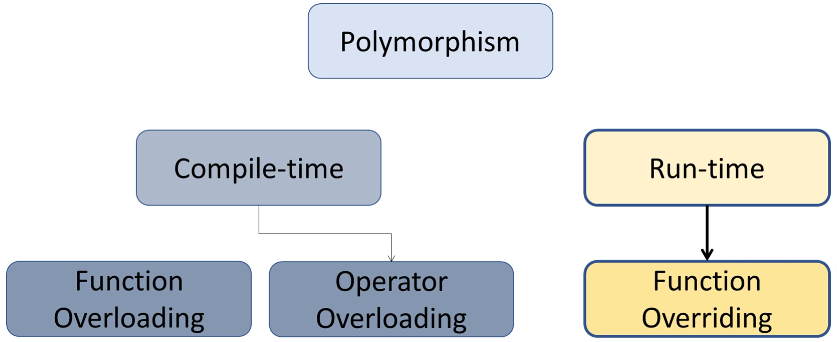
\includegraphics[width=\width\textwidth]{./figs/20220617211511.png}
    %\caption{}
\end{figure}
\begin{itemize}
    \item The best way to understand polymorphism is by using an example: let's think of a non-polymorphic example first.
        \begin{figure}[H]
            \centering
            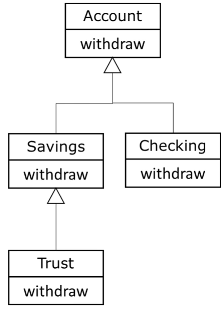
\includegraphics[width=\width\textwidth]{./figs/20220617211614.png}
            %\caption{}
        \end{figure}
        \begin{minted}[autogobble]{cpp}
            Account a;
            a.withdraw(1000); // Account::withdraw

            Savings b;
            b.withdraw(1000); // Savings::withdraw
            
            Checking c;
            c.withdraw(1000); // Checking::withdraw

            Trust d;
            d.withdraw(1000); // Trust::withdraw

            Account *p = new Trust();
            p->withdraw(1000); // Account::withdraw()
                               // Should be Trust::withdraw()
        \end{minted}
    
    \item See the problem? it is that the last exapmle gives a problem since we call the wrong function. So the static binding here is giving us problems.
    \item See another example:
        \begin{minted}[autogobble]{cpp}
            void display(const Account &acc) {
                acc.display();
                // will always use Account::display
            }
            Account a;
            display_account(a);

            Savings b;
            display_account(b);

            Checking c;
            display_account(c);

            Trust d;
            display_account(d);
        \end{minted}
        \begin{itemize}
            \item Now the problem is that the function parameter expects an account and will call the account's displayed method. This is the problem with static binding.
        \end{itemize}

    
    \item Now let's see the same example with dynamic polymorphism.
        \begin{itemize}
            \item Now withdraw is a virtual method in account.
        \end{itemize}
        \begin{minted}[autogobble]{cpp}
            Account a;
            a.withdraw(1000); // Account::withdraw

            Savings b;
            b.withdraw(1000); // Savings::withdraw
            
            Checking c;
            c.withdraw(1000); // Checking::withdraw

            Trust d;
            d.withdraw(1000); // Trust::withdraw

            Account *p = new Trust();
            p->withdraw(1000); // Trust::withdraw()
        \end{minted}
    
    \item Virtual methods allow the compiler to put the instructions necessary to check what kind of data the a pointer is pointing to and delegate the bindign to compilte time. Thus no more bugs.
    \item The same thing occurs when the above example is called using virtual methods.
        \begin{minted}[autogobble]{cpp}
            void display(const Account &acc) {
                acc.display();
                // will use the display method 
                // depending on what object is 
                // being pointed to at run time.
            }
            Account a;
            display_account(a);

            Savings b;
            display_account(b);

            Checking c;
            display_account(c);

            Trust d;
            display_account(d);
        \end{minted}
    
    \item This allows us to not duplicate code.
    \item With dynamic polymorphism we can define a function with a base class parameter and any class that derives from the base will get called the appropriate method name.
\end{itemize}

%%%%%%%%%%%%%%%%%%%%%%%%%%%%%%%%%%%%%%%%%%%%%%%%%%%%%%
\section{Polymorphism}
\begin{itemize}
    \item For dynamic polymorphism we must have:
        \begin{itemize}
            \item Inheritance
            \item Base class pointer or base class references
            \item virtual functions
        \end{itemize}
    
    \item Supose the following example has been implemented using dynamic polymorphism:
        \begin{minted}[autogobble]{cpp}
            Account *p1 = new Account();
            Account *p2 = new Savings();
            Account *p3 = new Checking();
            Account *p4 = new Trust();

            p1->withdraw(1000); // Account::withdraw
            p2->withdraw(1000); // Savings::withdraw
            p3->withdraw(1000); // Checking::withdraw
            p4->withdraw(1000); // Trust::withdraw

            // delete pointers
        \end{minted}
        \begin{figure}[H]
            \centering
            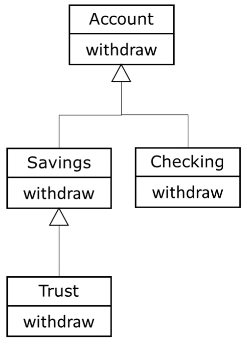
\includegraphics[width=\width\textwidth]{./figs/20220617214441.png}
            %\caption{}
        \end{figure}
    
    \item Now we suppose we want to create an array that holds pointers to accounts, we need dynamic polymorphism:
        \begin{minted}[autogobble]{cpp}
            Account *p1 = new Account();
            Account *p2 = new Savings();
            Account *p3 = new Checking();
            Account *p4 = new Trust();

            Account *array[] = {p1, p2, p3, p4};

            for (auto i = 0; i < 4; ++i) {
                array[i]->withdraw(1000);
            }
        \end{minted}
        \begin{figure}[H]
            \centering
            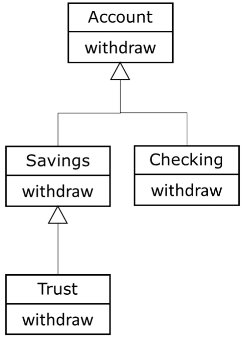
\includegraphics[width=\width\textwidth]{./figs/20220617214642.png}
            %\caption{}
        \end{figure}
        \begin{itemize}
            \item This allows us to program more abstractly.
            \item We simply withdraw 1000 from each of the accounts regardless of their specific type.
        \end{itemize}
\end{itemize}

%%%%%%%%%%%%%%%%%%%%%%%%%%%%%%%%%%%%%%%%%%%%%%%%%%%%%%
\section{Virtual functions}
\begin{itemize}
    \item Redfined functions are bound statically.
    \item Overridden functions are bound statically.
    \item Virtual functions are overriden.
    \item Allows us to treat all objects generally as objects of the base class.
\end{itemize}

\subsection{Declaring virtual functions}
\begin{itemize}
    \item Declare the function you want to override as virtual in the BASE class.
    \item Virtual functions are virtual all the way down the hierarchy from this point.
    \item Dynamic polymorphism only via account class poitner or reference.
        \begin{minted}[autogobble]{cpp}
            class Account {
                public:
                    virtual void withdraw(double amount);
            };
        \end{minted}
    
    \item Once we declare a function as virtual it is virtual in all the classes that inherit the base class from that point forward.
\end{itemize}


\subsection{Example}
\begin{itemize}
    \item Here is an example of a derived class that has a virtual method. 
    \item The method was declared virtual in the base so the virtual keyword in the derived classes are not necessary, but placing the keyword there is best practice.
        \begin{minted}[autogobble]{cpp}
            class Checking : public Account {
            public:
                virtual void withdraw(double amount);
            };
        \end{minted}
\end{itemize}

%%%%%%%%%%%%%%%%%%%%%%%%%%%%%%%%%%%%%%%%%%%%%%%%%%%%%%
\section{Virtual destructors}
\begin{itemize}
    \item Probelms can happen when we destroy polymorphic object.
    \item If a derived class is destroyed by deleting its storage via the base class pointer and the class a non-virtual destructor. Then the behavior is undefined in the C++ standard.
    \item Derived objects must be destroyed in the correct order starting at the correct destructor.
    \item There is a rule we can follow to avoid this:
        \begin{itemize}
            \item If a class has a virtual function, then always provide a public virtual destructor. 
            \item If a base class destructor is virtual then all derived class destructors are also virtual.
                \begin{minted}[autogobble]{cpp}
                    class Account {
                        public: virtual void withdraw(double amount);
                        virtual ~Account();
                    };
                \end{minted}
        \end{itemize}
    
    \item So the problem is that if we are inheriting methods the C++ language may call the base class method, making it virtual allows us to speicify to use the method of the current class not the base class.
\end{itemize}

%%%%%%%%%%%%%%%%%%%%%%%%%%%%%%%%%%%%%%%%%%%%%%%%%%%%%%
\section{Using the override specifier}
\begin{itemize}
    \item We can override base class virtual functions. 
    \item The function signature and return must be exactly the same. 
    \item If they are different then we have redefinition not overriding.
    \item Redefinition is statically bound. Overriding is dynamically bound.
    \item C++11 provides an override specifier to have the compiler ensure overriding.
    \item An example here is the following:
        \begin{itemize}
            \item The base class: \mintinline{cpp}{virtual void say_hello() const;} 
            \item The derived class: \mintinline{cpp}{virtual void say_hello();}
            \item Notice we forgot the const in the second one. C++ is dumb and thinks this is another different function, so it will consider it redefinition. We need to add the const to override.
            \item We can add the \mintinline{cpp}{override} keyword to specify that no matter what if the name of the method is the same as the method in the base class it must be overriden. This will merely print the error, it wont fix it, you will need to also make it const so its basically just a reminder.
        \end{itemize}
\end{itemize}

%%%%%%%%%%%%%%%%%%%%%%%%%%%%%%%%%%%%%%%%%%%%%%%%%%%%%%
\section{Using the final specifier}
\begin{itemize}
    \item C++11 provides the final specifier.
    \item When used at the class level it prevents a class form being derived from.
    \item When used at the method level it prevents virtual methods from being overriden in derived classes.
    \item Syntax in the class level: \begin{minted}[autogobble]{cpp}
        class my_class final {...};
    \end{minted}
    
    \item In this one we assume the base class is not final: \begin{minted}[autogobble]{cpp}
        class Derived final: public Base {...};
    \end{minted}
    
    \item Example of final methods:
        \begin{minted}[autogobble]{cpp}
            class A {
                public: virtual void do_something();
            };
            class B: public A {
                virtual void do_something() final; // no overriding further.
            };
            class C: public B {
                virtual void do_something(); // compiler error.
            };
        \end{minted}
\end{itemize}

%%%%%%%%%%%%%%%%%%%%%%%%%%%%%%%%%%%%%%%%%%%%%%%%%%%%%%
\section{Using base class references}
\begin{itemize}
    \item We can also use base class references with dynamic polymorphism. 
    \item This is useful when we pass objects to functions that expect a base class reference.
    \item In other words to make C++ do what everyone should expect it to do:
        \begin{minted}[autogobble]{cpp}
            Account a;
            Account &ref = a;
            ref.withdraw(10); // Account::withdraw

            Trust t;
            Account &ref1 = t;
            ref1.withdraw(10); // Trust::withdraw
        \end{minted}
    
    \item So for example we want to write a withdraw method that accepts all objects derived from Account, since its withdrawing, just subtracting from some attribute, it should work and call the appropriate withdraw method. So the following example works dinamically i.e. calling the appropriate withdraw method and not just the Account::withdraw.
        \begin{minted}[autogobble]{cpp}
            void do_withdraw(Account &account, double amount) {
                account.withdraw(amount);
            }
            Account a;
            do_withdraw(a, 1000); // Account::withdraw

            Trust t; 
            do_withdraw(t, 1000); // Trust::withdraw
        \end{minted}
\end{itemize}

%%%%%%%%%%%%%%%%%%%%%%%%%%%%%%%%%%%%%%%%%%%%%%%%%%%%%%
\section{Pure virtual functions and abstract classes}
\begin{itemize}
    \item Abstract class:
        \begin{itemize}
            \item Cannot instantiate object.
            \item These classes are used as base classes in inheritance hiearchies.
            \item Often refered to as abstract base classes.
        \end{itemize}
    
    \item Concrete class:
        \begin{itemize}
            \item These classes can instantiate objects.
            \item All their member funtions are defined, in short, the ones we have been using up until this point in the course.
        \end{itemize}
\end{itemize}

\subsection{Polymorphism}
Pure virtual functions and obstract classes.
\begin{itemize}
    \item Abstract base class:
        \begin{itemize}
            \item Too generic to create objects from: shape, employee, account, player.
            \item Serves as parent to derived classes that me have objects.
            \item Contains at least one pure virtual function.
            \item Can be thought out as a parent class to other classes.
        \end{itemize}
    
    \item What is a pure virtual function:
        \begin{itemize}
            \item Used to make a class abstract.
            \item Specified with ''=0´´ in its declaration.
                \begin{minted}[autogobble]{cpp}
                    virtual void function() = 0; // pure virtual function.
                \end{minted}
            
            \item Typically do not provide implementations. So no \mintinline{cpp}|{code...}| curly braces, or implementation usually, however we can implement some functionality.
            \item Once a class has at least one virtual function, it is now an abstract class and cannot be instantiated.
        \end{itemize}
    
    \item Pure virtual functions and abstract classes:
        \begin{itemize}
            \item Virtual functions must be override the base class.
            \item If the derived class does not override the derived class is also abstract and therefore cannot be instantiated.
            \item Used when it doesn't make sense for a base class to have an implementation:
                \begin{itemize}
                    \item But concrete classes must implement it.
                \end{itemize}
            \begin{minted}[autogobble]{cpp}
                virtual void draw() = 0; // Shape
                virtual void defend() = 0; // Player
            \end{minted}
        \end{itemize}
    
    \item So why have an abstract class?
        \begin{itemize}
            \item Say we are creating a class called shape. At the moment we know that shapes can be of all types, triangle, square, parallelogram, but we know that these shapes all will need a draw() method. So what we can do is create an abstract class called Shape, and define a virtual draw method, then create all the class variations and inherit from the parent. We must always override the draw() method, otherwise it is inherited as virtual and makes the derived class also abstract.
                \begin{figure}[H]
                    \centering
                    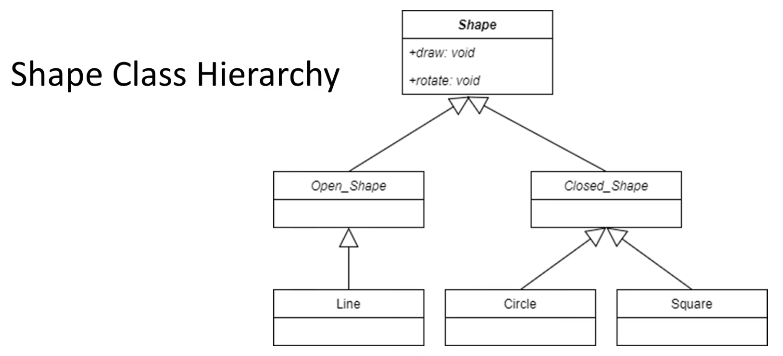
\includegraphics[width=\width\textwidth]{./figs/20230204190832.png}
                    %\caption{}
                \end{figure}
            
            \item Here some code for the shape class:
                \begin{minted}[autogobble]{cpp}
                    class Shape {
                        private:    
                            // attributes commont to all shapes.
                        public:
                            virtual void draw() = 0; // pure virtual function.
                            virtual void rotate() = 0; // pure virtual function.
                            virtual ~Shape(); // pure virtual function.
                            ...
                    };
                    class Circle : public Shape { // Concrete class.
                        private:
                            // attributes for a circle.
                        public:
                            virtual void draw() override {
                                // code to draw a circle.
                            }
                            virtual void rotate() override {
                                // code to rotate a circle.
                            }
                            virtual ~Circle;
                            ...
                    };
                \end{minted}
            
            \item If we try to instantiate the abstract class we get an error:
                \begin{minted}[autogobble]{cpp}
                    Shape shape;              // Error.
                    Shape *ptr = new Shape(); // Error.
                \end{minted}
            
            \item We can use pointers and refernces to dynamically refer to concrete classes derived from them. Example:
                \begin{minted}[autogobble]{cpp}
                    Shape *ptr = new Circle(); // OK.
                    ptr->draw();
                    ptr->rotate();
                \end{minted}
        \end{itemize}
\end{itemize}

%%%%%%%%%%%%%%%%%%%%%%%%%%%%%%%%%%%%%%%%%%%%%%%%%%%%%%
\section{Polymorphism}
\begin{itemize}
    \item What does it mean to use a class as an interface?
        \begin{itemize}
            \item An abstract class that has only pure virtual functions.
            \item These functions provide a general set of services to the other user of the class.
            \item Provided as public. These methods need to be public.
            \item Each subclass is free to implement these services as needed.
            \item Every service (by service we just mean method) must be implemented.
            \item The service type information is strictly enforced.
        \end{itemize}
    
    \item A printable example:
        \begin{itemize}
            \item C++ does not provide true interfaces.
            \item We use abstract classes and pure virtual functions to achieve it.
            \item We suppose we want to be able to printable support for any object we wish without knowing its implementation at compile time.
                \begin{minted}[autogobble]{cpp}
                    std::cout << any_object << std::endl;
                \end{minted}
            
            \item \mintinline{cpp}{any_object} must comform to the printable interface.
            \item So for this example we want to create an abstract class that gives all derived classes the capacity to print themselves.
                \begin{minted}[autogobble]{cpp}
                    class Printable {
                            friend ostream &operator<<(ostream &os, Printable &obj);
                        public:
                            virtual void print(ostream &os) const = 0;
                            virtual ~Printable() {};
                            ...
                    };
                    ostream &operator<<(ostream &os, const Printable &obj) {
                        obj.print(os);
                        return os;
                    }
                \end{minted}
            
            \item So for any class to get the services from the Printable class it must override the Printable::print() method implemented in the Printable class.
            
            \item So things like this work:
                \begin{minted}[autogobble]{cpp}
                    Any_class *ptr = new Any_class();
                    cout << *ptr << endl;

                    void function1(Any_class &obj) {
                        cout << obj << endl;
                    }
                    void function2(Printable &obj) {
                        cout << obj << endl;
                    }

                    function1(*ptr); // "Hi from Any_class"
                    function2(*ptr); // "Hi from Any_class"
                \end{minted}
            
            \item function1 and function2 will be exactly the same, since Any\_class is a printable so it works on function 2 and Any\_class is also an Any\_class, so it works on function 1.
        \end{itemize}
    
    \item Usually when a class is intended to be used as an interface it is preceded by I\_ to indicate that this is intended as an interface.
\end{itemize}

\subsection{Example code}
\begin{minted}[autogobble]{cpp}
    #include <iostream>
    class I_Printable {
            friend std::ostream &operator<<(std::ostream &os, const I_Printable &obj);
        public:
        virtual void print(std::ostream &os) const = 0;
        virtual ~I_Printable() {};
    };
    std::ostream &operator<<(std::ostream &os, const I_Printable &obj) {
        obj.print(os);
        return os;
    }
    class Account : public I_Printable {
        public:
        virtual void withdraw(double amount) {
            std::cout << "In Account::withdraw" << std::endl;
        }
        virtual void print(std::ostream &os) const override {
            os << "Account display";
        }
        virtual ~Account() {  }
    };
    class Checking: public Account  {
        public:
        virtual void withdraw(double amount) {
            std::cout << "In Checking::withdraw" << std::endl;
        }
        virtual void print(std::ostream &os) const override {
            os << "Checking display";
        }
        virtual ~Checking() {  }
    };
    class Savings: public Account {
        public:
        virtual void withdraw(double amount) {
            std::cout << "In Savings::withdraw" << std::endl;
        }
        virtual void print(std::ostream &os) const override {
            os << "Savings display";
        }
        virtual ~Savings() {  }
    };
    class Trust: public Account  {
    public:
        virtual void withdraw(double amount) {
            std::cout << "In Trust::withdraw" << std::endl;
        }
        virtual void print(std::ostream &os) const override {
            os << "Trust display";
        }
        virtual ~Trust() {  }
    };
    class Dog : public I_Printable {
    public:
    virtual void print(std::ostream &os) const override {
            os << "Woof woof";
        } 
    };
    void print(const I_Printable &obj) {
        std::cout << obj << std::endl;
    }
    int main() {
        
        Dog *dog = new Dog();
        std::cout << *dog<< std::endl;  
        
        print(*dog);
        
        Account *p1 = new Account();
        std::cout << *p1<< std::endl;
            
        Account *p2 = new Checking();
        std::cout << *p2<< std::endl;  

        delete p1;
        delete p2;
        delete dog;
        return 0;
    }
    /* Output:
    Woof woof
    Woof woof
    Account display
    Checking display
    */
\end{minted}

%%%%%%%%%%%%%%%%%%%%%%%%%%%%%%%%%%%%%%%%%%%%%%%%%%%%%%
\section{Section challenge}